\chapter{Funkcje rzeczywiste analityczne}
\label{ma2:ch:real-analytic}

W rozdziale \ref{ma2:ch:power-series} badaliśmy
zbieżność szeregów potęgowych jednej zmiennej,
a w rozdziale \ref{ma2:ch:taylor} otrzymaliśmy
wzory Taylora skończonego rzędu.
Teraz rozważymy pytanie, kiedy funkcję można
odtworzyć z jej pochodnych wszystkich rzędów.
Rozróżnienie gładkości i analityczności jest
zasadnicze: istnienie wszystkich pochodnych
nie gwarantuje jeszcze, że ich wartości
w jednym punkcie wyznaczają funkcję w otoczeniu.

\section{Analityczność jednej zmiennej}

\begin{definicja}
\label{ma2:def:real-analytic-one}
Niech $I\subseteq\R$ będzie zbiorem otwartym.
Funkcja $f:I\to\R$ jest rzeczywista analityczna
w punkcie $a\in I$, jeżeli istnieje $r>0$
takie, że $(a-r,a+r)\subseteq I$ oraz
istnieją liczby $c_j$ spełniające
\[
 f(a+h)=\sum_{j=0}^\infty c_jh^j,\qquad |h|<r.
\]
Funkcja jest analityczna na $I$, gdy jest
analityczna w każdym jego punkcie.
Klasę takich funkcji oznaczamy $C^\omega(I)$.
\end{definicja}

\begin{stwierdzenie}
\label{ma2:prop:analytic-taylor-one}
Jeżeli $f$ jest analityczna w $a$, to
jest gładka w pewnym otoczeniu $a$, a jej
rozwinięcie jest jednoznaczne i ma postać
\[
 f(a+h)=\sum_{j=0}^\infty
 \frac{f^{(j)}(a)}{j!}h^j.
\]
\end{stwierdzenie}
\begin{proof}
Różniczkujemy szereg potęgowy dowolną
skończoną liczbę razy wewnątrz jego przedziału
zbieżności, stosując
\ref{ma2:thm:power-derivative-radius}
oraz \ref{ma2:thm:power-derivative}.
Po podstawieniu $h=0$ otrzymujemy
$f^{(j)}(a)=j!c_j$.
Jednoznaczność jest również treścią
\ref{ma2:cor:power-coefficients}.
\end{proof}

\begin{stwierdzenie}[Kryterium reszty Taylora]
\label{ma2:prop:analytic-taylor-remainder}
Niech $f$ będzie klasy $C^\infty$ w otoczeniu $a$.
Funkcja jest analityczna w $a$ wtedy i tylko wtedy,
gdy dla pewnego $r>0$ i wszystkich $|h|<r$
zachodzi
\[
 \lim_{N\to\infty}
 \left(f(a+h)-\sum_{j=0}^N
 \frac{f^{(j)}(a)}{j!}h^j\right)=0.
\]
\end{stwierdzenie}
\begin{proof}
Warunek jest dokładnie warunkiem zbieżności
sum częściowych szeregu Taylora do funkcji.
Konieczność wynika z
\ref{ma2:prop:analytic-taylor-one},
a dostateczność z definicji
\ref{ma2:def:real-analytic-one}.
\end{proof}

\begin{twierdzenie}[Kryterium oszacowań pochodnych]
\label{ma2:thm:analytic-derivative-bound}
Niech $f$ będzie klasy $C^\infty$
na $(a-r,a+r)$, gdzie $r>0$.
Jeżeli istnieją $C,A>0$ takie, że
\[
 |f^{(j)}(x)|\le C A^j j!
 \qquad (j\ge0,\ |x-a|<r),
\]
to $f$ jest analityczna na tym przedziale.
\end{twierdzenie}
\begin{proof}
Ustalmy $b\in(a-r,a+r)$ i wybierzmy
$0<\delta<\min\{r-|b-a|,1/A\}$.
Dla $|h|<\delta$ cały odcinek od $b$ do $b+h$
leży w dziedzinie podanego oszacowania.
Z reszty Lagrange'a
(\ref{ma2:thm:taylor-lagrange}) otrzymujemy
\[
 \left|f(b+h)-\sum_{j=0}^N
 \frac{f^{(j)}(b)}{j!}h^j\right|
 \le C(A|h|)^{N+1}.
\]
Prawa strona dąży do zera, ponieważ $A|h|<1$.
Stosujemy \ref{ma2:prop:analytic-taylor-remainder}.
\end{proof}

\begin{przyklad}[Funkcja gładka, lecz nieanalityczna]
\label{ma2:ex:analytic-flat}
Niech
\[
 f(x)=
 \begin{cases}
 \exp(-1/x^2),&x\ne0,\\
 0,&x=0.
 \end{cases}
\]
Dla $x\ne0$ każda pochodna ma postać
$f^{(j)}(x)=P_j(1/x)\exp(-1/x^2)$
z pewnym wielomianem $P_j$.
Istotnie, $P_0=1$, a różniczkowanie daje
\[
 P_{j+1}(t)=-t^2 P_j'(t)+2t^3P_j(t).
\]
Dla dowolnego całkowitego $m\ge0$
mamy $|t|^m\exp(-t^2)\to0$ przy $|t|\to\infty$:
na przykład z szeregu wykładniczego
$\exp(t^2)\ge t^{2N}/N!$ dla $2N>m$.
Indukcyjnie $f^{(j)}(0)=0$ dla wszystkich $j$,
gdyż iloraz różnicowy w zerze także jest
wielomianem w $1/x$ pomnożonym przez
$\exp(-1/x^2)$ i ma granicę zero.
Ta sama granica zapewnia ciągłość każdej
pochodnej w zerze.
Szereg Taylora w zerze jest więc tożsamościowo
zerowy, lecz $f(x)>0$ dla $x\ne0$.
Funkcja nie jest analityczna w zerze.
\end{przyklad}

\begin{figure}[htbp]
\centering
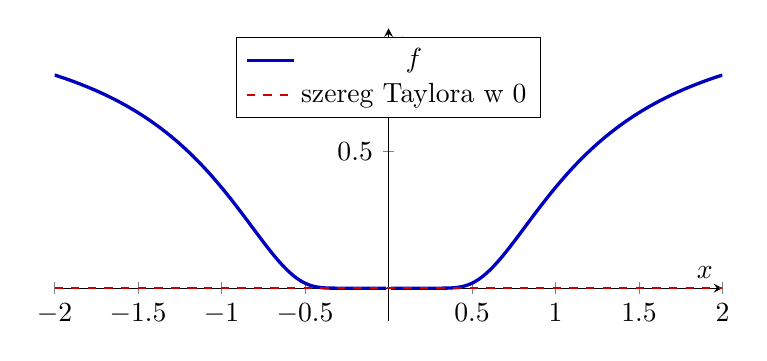
\begin{tikzpicture}
\begin{axis}[width=.83\linewidth,height=5.3cm,
 axis lines=middle,xlabel={$x$},ylabel={$y$},
 xmin=-2,xmax=2,ymin=-.12,ymax=.95,
 domain=-2:2,samples=200,
 legend style={at={(.5,.97)},anchor=north}]
\addplot[blue!75!black,very thick,domain=-2:-.015] {exp(-1/(x*x))};
\addlegendentry{$f$}
\addplot[blue!75!black,very thick,domain=.015:2,forget plot] {exp(-1/(x*x))};
\addplot[red!80!black,dashed,thick] {0};
\addlegendentry{szereg Taylora w $0$}
\end{axis}
\end{tikzpicture}
\caption{Wszystkie pochodne funkcji $f$ w zerze
znikają, chociaż funkcja jest dodatnia poza zerem.}
\label{ma2:fig:analytic-flat}
\end{figure}

\section{Szeregi potęgowe wielu zmiennych}

Dla wielowskaźnika $\alpha=(\alpha_1,\ldots,\alpha_n)
\in\N_0^n$ stosujemy oznaczenia
$|\alpha|=\sum_i\alpha_i$,
$\alpha!=\prod_i\alpha_i!$,
$h^\alpha=\prod_i h_i^{\alpha_i}$
oraz $\partial^\alpha=\partial_1^{\alpha_1}
\cdots\partial_n^{\alpha_n}$, zgodnie
z rozdziałem \ref{ma2:ch:taylor}.
Przyjmujemy $\N_0=\{0,1,\ldots\}$.
Dla $r>0$ niech $Q_r=\{h\in\R^n:\|h\|_\infty<r\}$.

\begin{definicja}
\label{ma2:def:analytic-multi}
Niech $U\subseteq\R^n$ będzie otwarty.
Funkcja $f:U\to\R$ jest analityczna w $a\in U$,
jeżeli dla pewnego $r>0$, $a+Q_r\subseteq U$,
istnieje rodzina współczynników
$(c_\alpha)_{\alpha\in\N_0^n}$ taka, że
\[
 \sum_\alpha |c_\alpha|r^{|\alpha|}<\infty,
 \qquad
 f(a+h)=\sum_\alpha c_\alpha h^\alpha
 \quad (h\in Q_r).
\]
Analityczność na $U$ oznacza analityczność
w każdym punkcie $U$.
Odwzorowanie $f:U\to\R^m$ jest analityczne,
gdy każda jego składowa jest analityczna.
\end{definicja}

Wybór sześcianu zamiast kuli nie zmienia
lokalnego charakteru definicji:
każde otoczenie punktu zawiera taki sześcian.
Wymaganie sumowalności przy promieniu $r$
nie jest warunkiem zbieżności na maksymalnym
obszarze szeregu. Jeśli szereg jest bezwzględnie
zbieżny w pewnym otwartym sześcianie,
to wystarczy zmniejszyć jego promień
i sprawdzić bezwzględną zbieżność
w punkcie $(r,\ldots,r)$.

\begin{twierdzenie}[Różniczkowanie szeregu wielowymiarowego]
\label{ma2:thm:analytic-multi-derivative}
Jeżeli $\sum_\alpha |c_\alpha|r^{|\alpha|}<\infty$,
to szereg $\sum_\alpha c_\alpha h^\alpha$
oraz wszystkie szeregi otrzymane przez
różniczkowanie wyraz po wyrazie dowolnego
skończonego rzędu są jednostajnie
i bezwzględnie zbieżne na każdym domkniętym
sześcianie $\overline{Q_s}$, $0<s<r$.
Suma $f$ jest klasy $C^\infty$ na $Q_r$,
a dla każdego wielowskaźnika $\beta$
\[
 \partial^\beta f(h)=
 \sum_{\alpha\ge\beta} c_\alpha
 \frac{\alpha!}{(\alpha-\beta)!}h^{\alpha-\beta}.
\]
Nierówność $\alpha\ge\beta$ rozumiemy współrzędnościowo.
\end{twierdzenie}
\begin{proof}
Ustalmy $\beta$ i $s\in(0,r)$.
Dla $|\beta|=m\ge1$ i $\alpha\ge\beta$
mamy $\alpha!/(\alpha-\beta)!\le|\alpha|^m$,
gdyż iloczyn zawiera $m$ czynników,
z których żaden nie przekracza $|\alpha|$.
Zatem dla $\|h\|_\infty\le s$
\[
 \left|c_\alpha\frac{\alpha!}{(\alpha-\beta)!}
 h^{\alpha-\beta}\right|
 \le |c_\alpha|r^{|\alpha|}
 s^{-m}|\alpha|^m(s/r)^{|\alpha|}.
\]
Ciąg $l^m(s/r)^l$ jest ograniczony:
dla $l\ge1$ iloraz kolejnych wyrazów
dąży do $s/r<1$.
Dla $m=0$ stosujemy bezpośrednio
$|h^\alpha|\le r^{|\alpha|}$.
Kryterium Weierstrassa daje więc
jednostajną zbieżność bezwzględną.
Uporządkujmy sumy częściowe według stopnia
całkowitego $|\alpha|$ (na każdym stopniu
jest skończenie wiele wielowskaźników).
Są to wielomiany, a ich pochodne
wszystkich ustalonych rzędów mają
jednostajne granice na mniejszych sześcianach.
Stosując twierdzenie o różniczkowaniu
granicy jednostajnej do każdej zmiennej
osobno, na odcinkach równoległych do osi,
a następnie indukcyjnie do pochodnych,
otrzymujemy podany wzór.
Jednostajna zbieżność ciągłych funkcji
zapewnia ciągłość pochodnych.
Każdy punkt $Q_r$ należy do wnętrza
pewnego takiego mniejszego sześcianu.
\end{proof}

\begin{wniosek}[Jednoznaczność szeregu Taylora]
\label{ma2:cor:analytic-multi-coefficients}
Jeżeli $f$ jest analityczna w $a$, to jest
gładka w otoczeniu $a$ oraz
\[
 c_\alpha=\frac{\partial^\alpha f(a)}{\alpha!}.
\]
W szczególności rozwinięcie jest jednoznaczne.
\end{wniosek}
\begin{proof}
Stosujemy \ref{ma2:thm:analytic-multi-derivative}
do funkcji $h\mapsto f(a+h)$ i podstawiamy $h=0$.
W szeregu pochodnej rzędu $\alpha$ pozostaje
jedynie wyraz o indeksie $\alpha$.
\end{proof}

\section{Zmiana środka rozwinięcia}

\begin{twierdzenie}[Przesunięcie środka szeregu]
\label{ma2:thm:analytic-recenter}
Niech $f(a+h)=\sum_\alpha c_\alpha h^\alpha$
dla $h\in Q_r$, gdzie
$\sum_\alpha |c_\alpha|r^{|\alpha|}<\infty$.
Jeżeli $b=a+v$ i $\|v\|_\infty<r$, to dla
$0<s<r-\|v\|_\infty$ zachodzi
\[
 f(b+w)=\sum_\beta d_\beta w^\beta
 \quad(w\in Q_s),\qquad
 d_\beta=\sum_{\alpha\ge\beta}
 \binom{\alpha}{\beta}c_\alpha v^{\alpha-\beta},
\]
gdzie $\binom{\alpha}{\beta}
=\prod_{i=1}^n\binom{\alpha_i}{\beta_i}$.
Ponadto $\sum_\beta |d_\beta|s^{|\beta|}<\infty$.
W szczególności suma szeregu jest analityczna
na całym $a+Q_r$.
\end{twierdzenie}
\begin{proof}
Stosujemy wzór dwumianowy do każdej współrzędnej:
\[
 (v+w)^\alpha
 =\sum_{\beta\le\alpha}\binom{\alpha}{\beta}
 v^{\alpha-\beta}w^\beta.
\]
Sumowalność rodziny powstałej po rozwinięciu
wynika z oszacowania
\[
 \begin{aligned}
 &\sum_\alpha |c_\alpha|
 \sum_{\beta\le\alpha}\binom{\alpha}{\beta}
 |v^{\alpha-\beta}|s^{|\beta|}\\
 &\qquad=\sum_\alpha |c_\alpha|
 \prod_{i=1}^n(|v_i|+s)^{\alpha_i}
 \le\sum_\alpha |c_\alpha|r^{|\alpha|}<\infty .
 \end{aligned}
\]
Możemy więc zmienić kolejność sumowania
i pogrupować wyrazy według potęg $w^\beta$.
To daje wzór na $d_\beta$ oraz
$\sum_\beta|d_\beta|s^{|\beta|}
\le\sum_\alpha|c_\alpha|r^{|\alpha|}$.
Jednoznaczność z
\ref{ma2:cor:analytic-multi-coefficients}
pokazuje także, że
$d_\beta=\partial^\beta f(b)/\beta!$.
\end{proof}

\begin{wniosek}[Lokalne oszacowania wszystkich pochodnych]
\label{ma2:cor:analytic-local-derivative-bound}
Jeżeli $f$ jest analityczna w $a\in\R^n$,
to istnieją $s,C,A>0$ takie, że
\[
 |\partial^\beta f(x)|\le C A^{|\beta|}\beta!
 \qquad(x\in a+Q_s,\ \beta\in\N_0^n).
\]
\end{wniosek}
\begin{proof}
Wybieramy rozwinięcie z
\ref{ma2:def:analytic-multi} o promieniu $r$.
Przyjmijmy $s=r/3$ i
$C=1+\sum_\alpha|c_\alpha|r^{|\alpha|}$.
Dla $x=a+v\in a+Q_s$ dowód
\ref{ma2:thm:analytic-recenter} daje
$\sum_\beta |d_\beta|s^{|\beta|}\le C$.
Stąd $|d_\beta|\le Cs^{-|\beta|}$.
Ponieważ $d_\beta=\partial^\beta f(x)/\beta!$,
wystarczy przyjąć $A=1/s$.
\end{proof}

\begin{twierdzenie}[Wielowymiarowe kryterium analityczności]
\label{ma2:thm:analytic-multi-bound}
Niech $f$ będzie klasy $C^\infty$ na $a+Q_r$.
Jeżeli dla pewnych $C,A>0$ zachodzi
\[
 |\partial^\beta f(x)|\le C A^{|\beta|}\beta!
 \qquad(x\in a+Q_r,\ \beta\in\N_0^n),
\]
to $f$ jest analityczna na $a+Q_r$.
\end{twierdzenie}
\begin{proof}
Ustalmy $b\in a+Q_r$ i wybierzmy
$0<s<\min\{r-\|b-a\|_\infty,1/(nA)\}$.
Dla $h\in Q_s$ rozważamy funkcję
$g(t)=f(b+th)$ na otoczeniu $[0,1]$.
Wielokrotne zastosowanie reguły łańcuchowej
i wzoru wielomianowego daje
\[
 g^{(j)}(t)=\sum_{|\alpha|=j}
 \frac{j!}{\alpha!}\partial^\alpha f(b+th)h^\alpha.
\]
Wzór wynika też z wielowskaźnikowej postaci
pochodnej w \ref{ma2:cor:taylor-multiindex}.
Zatem dla $t\in[0,1]$,
\[
 \frac{|g^{(j)}(t)|}{j!}
 \le C A^j\sum_{|\alpha|=j}|h^\alpha|
 \le C(nA\|h\|_\infty)^j.
\]
Ostatnia nierówność wynika z rozwinięcia
$(|h_1|+\cdots+|h_n|)^j$, w którym każdy
współczynnik wielomianowy jest co najmniej $1$.
Z reszty Lagrange'a
(\ref{ma2:thm:taylor-lagrange}) wynika więc
\[
 \left|f(b+h)-\sum_{|\alpha|\le N}
 \frac{\partial^\alpha f(b)}{\alpha!}h^\alpha\right|
 \le C(nA\|h\|_\infty)^{N+1}.
\]
Prawa strona dąży do zera.
Dla współczynników
$c_\alpha=\partial^\alpha f(b)/\alpha!$
mamy ponadto
\[
 \sum_\alpha |c_\alpha|s^{|\alpha|}
 \le C\sum_{j=0}^\infty (nAs)^j<\infty,
\]
gdyż liczba wielowskaźników stopnia $j$
jest nie większa od $n^j$ (każdy jest
licznikiem wystąpień liter w pewnym słowie
długości $j$ nad alfabetem $n$-elementowym).
Spełnione są zatem oba warunki definicji
\ref{ma2:def:analytic-multi}.
\end{proof}

\section{Działania na funkcjach analitycznych}

W poniższych dowodach użyteczny będzie
rachunek szeregów z bezwzględnie sumowalnymi
współczynnikami. Dla $r>0$ oznaczmy przez
$\mathcal A_r^{(n)}$ przestrzeń rzeczywistych rodzin
$c=(c_\alpha)_{\alpha\in\N_0^n}$ takich, że
\[
 \|c\|_r=\sum_\alpha |c_\alpha|r^{|\alpha|}<\infty.
\]
Rodzinę utożsamiamy z szeregiem $\sum_\alpha c_\alpha h^\alpha$.
Nie utożsamiamy natomiast normy $\|\cdot\|_r$
z normą supremum sumy tego szeregu.

\begin{lemat}[Norma współczynników i iloczyn Cauchy'ego]
\label{ma2:lem:analytic-series-algebra}
Przestrzeń $\mathcal A_r^{(n)}$ z normą
$\|\cdot\|_r$ jest zupełna.
Iloczyn określony wzorem
\[
 (cd)_\gamma=\sum_{\alpha+\beta=\gamma}c_\alpha d_\beta
\]
należy do tej samej przestrzeni i spełnia
$\|cd\|_r\le\|c\|_r\|d\|_r$.
Jego suma na $Q_r$ jest iloczynem sum
szeregów $c$ i $d$.
\end{lemat}
\begin{proof}
Odwzorowanie $(c_\alpha)\mapsto
(r^{|\alpha|}c_\alpha)$ jest liniową izometrią
na przestrzeń $\ell^1(\N_0^n)$, która jest zupełna.
Dla każdego $\gamma$ w definicji iloczynu
występuje skończenie wiele par indeksów.
Sumowanie nieujemnych wyrazów daje
\[
 \begin{aligned}
 \|cd\|_r
 &\le \sum_{\alpha,\beta}|c_\alpha||d_\beta|
 r^{|\alpha|+|\beta|}\\
 &=\|c\|_r\|d\|_r .
 \end{aligned}
\]
Dla $h\in Q_r$ rodzina
$(c_\alpha d_\beta h^{\alpha+\beta})_{\alpha,\beta}$
jest bezwzględnie sumowalna na mocy
tego samego oszacowania.
Grupowanie według $\gamma=\alpha+\beta$
daje tożsamość dla sum szeregów.
\end{proof}

\begin{wniosek}
\label{ma2:cor:analytic-algebra}
Jeżeli $f,g:U\to\R$ są analityczne, to
$f+g$, $fg$, wszystkie pochodne cząstkowe $f$
oraz $\xi f$ dla $\xi\in\R$ są analityczne.
Funkcja $1/f$ jest analityczna na zbiorze
$\{x\in U:f(x)\ne0\}$.
\end{wniosek}
\begin{proof}
W ustalonym punkcie $a$ wybieramy wspólny
promień rozwinięć, zmniejszając w razie potrzeby
promienie obu szeregów.
Suma i mnożenie przez skalar zachowują
bezwzględną sumowalność współczynników,
a dla iloczynu stosujemy
\ref{ma2:lem:analytic-series-algebra}.
Różniczkowanie zachowuje tę własność
na każdym mniejszym sześcianie dzięki
oszacowaniom z
\ref{ma2:thm:analytic-multi-derivative}.

Jeżeli $f(a)\ne0$, piszemy
$f(a+h)=f(a)(1-u(h))$, gdzie $u(0)=0$.
Szereg $u$ ma zerowy wyraz stały.
Jeżeli ma skończoną normę przy promieniu $r$,
to przy $0<s<r$ zachodzi
\[
 \|u\|_s\le(s/r)\|u\|_r.
\]
Wybieramy $s$ tak małe, by $\|u\|_s<1$.
Z submultiplikatywności normy
i zupełności przestrzeni
$\mathcal A_s^{(n)}$ wynika zbieżność
szeregu $\sum_{j=0}^\infty u^j$ w tej przestrzeni:
suma norm jest ograniczona przez
$\sum_{j=0}^\infty\|u\|_s^j$.
Dla każdego $h\in Q_s$ mamy
$|u(h)|\le\|u\|_s<1$, więc suma
jest równa $1/(1-u(h))$.
Istotnie, wartości sum częściowych zbiegają
do wartości szeregu granicznego, gdyż
$|v(h)|\le\|v\|_s$ dla każdego szeregu $v$.
Po podzieleniu przez $f(a)$ otrzymujemy
analityczność odwrotności w punkcie $a$.
\end{proof}

\begin{twierdzenie}[Złożenie odwzorowań analitycznych]
\label{ma2:thm:analytic-composition}
Niech $U\subseteq\R^n$, $V\subseteq\R^m$
będą otwarte, a $g:U\to V$ i $f:V\to\R^p$
odwzorowaniami analitycznymi.
Wtedy $f\circ g$ jest analityczne na $U$.
\end{twierdzenie}
\begin{proof}
Wystarczy rozważyć jedną składową $f$.
Ustalmy $a\in U$ oraz $b=g(a)$.
Dla pewnego $r>0$ mamy rozwinięcie
$f(b+z)=\sum_{\alpha\in\N_0^m}c_\alpha z^\alpha$
z $\sum_\alpha|c_\alpha|r^{|\alpha|}<\infty$.
Dla składowych $g$ piszemy
$g_i(a+h)=b_i+u_i(h)$.
Każdy szereg $u_i$ ma zerowy wyraz stały.
Z poprzedniego dowodu wynika, że
$\|u_i\|_s\to0$ przy $s\to0^+$.
Wybieramy wspólny promień $s$ tak mały,
aby $\|u_i\|_s<r$ dla wszystkich $i$
i $a+Q_s\subseteq U$.
W przestrzeni $\mathcal A_s^{(n)}$ mamy
\[
 \sum_\alpha\left\|c_\alpha
 \prod_{i=1}^m u_i^{\alpha_i}\right\|_s
 \le \sum_\alpha |c_\alpha|r^{|\alpha|}<\infty
\]
na mocy \ref{ma2:lem:analytic-series-algebra}.
Zupełność daje zatem sumę będącą
szeregiem potęgowym w $h$.
Dla $h\in Q_s$ wartość szeregu jest
równa $f(g(a+h))$, ponieważ ewaluacja
$u\mapsto u(h)$ jest ciągła względem
$\|\cdot\|_s$ i zachowuje iloczyny.
To dowodzi tezy w punkcie $a$.
\end{proof}

\section{Twierdzenie o identyczności}

\begin{twierdzenie}[Twierdzenie o identyczności]
\label{ma2:thm:analytic-identity}
Niech $U\subseteq\R^n$ będzie spójnym zbiorem
otwartym, a $f,g:U\to\R$ funkcjami analitycznymi.
Jeżeli $f=g$ na pewnym niepustym otwartym
podzbiorze $U$, to $f=g$ na całym $U$.
To samo zachodzi, jeśli dla pewnego $a\in U$
wszystkie pochodne cząstkowe $f$ i $g$
(w tym pochodne rzędu zero) są równe w $a$.
\end{twierdzenie}
\begin{proof}
Niech $u=f-g$, co jest funkcją analityczną
na mocy \ref{ma2:cor:analytic-algebra}.
Rozważmy zbiór
\[
 Z=\{x\in U:\partial^\alpha u(x)=0
                   \text{ dla każdego }\alpha\in\N_0^n\}.
\]
Jest względnie domknięty w $U$ jako
przecięcie zbiorów zerowych ciągłych funkcji.
Jeżeli $x\in Z$, to wszystkie współczynniki
rozwinięcia $u$ w $x$ są zerowe, na mocy
\ref{ma2:cor:analytic-multi-coefficients}.
Funkcja $u$ jest więc zerowa w otoczeniu $x$,
a w tym otoczeniu znikają również wszystkie
jej pochodne. Zatem $Z$ jest względnie otwarty.
Każde z założeń twierdzenia zapewnia,
że $Z$ jest niepusty.
Spójność $U$ daje $Z=U$, a w szczególności
$u=0$ na $U$.
\end{proof}

\begin{wniosek}[Izolowane zera w jednej zmiennej]
\label{ma2:cor:analytic-isolated-zeros}
Niech $I$ będzie otwartym przedziałem,
a $f:I\to\R$ funkcją analityczną,
która nie jest tożsamościowo zerowa.
Każde jej zero $a$ jest izolowane i ma
skończony rząd: istnieje $m\ge1$ i funkcja
$g$ analityczna w otoczeniu $a$, $g(a)\ne0$,
takie że $f(x)=(x-a)^m g(x)$.
\end{wniosek}
\begin{proof}
Gdyby wszystkie pochodne w $a$ były zerowe,
to \ref{ma2:thm:analytic-identity} dawałoby
$f=0$ na $I$. Istnieje więc najmniejszy
indeks $m\ge1$ z $c_m=f^{(m)}(a)/m!\ne0$.
W rozwinięciu w $a$ wyłączamy czynnik
$(x-a)^m$; pozostały szereg jest zbieżny
w tym samym otwartym przedziale zbieżności,
gdyż przy każdym dodatnim mniejszym promieniu
jego suma modułów jest sumą modułów ogona
pierwotnego szeregu podzieloną przez
promień podniesiony do potęgi $m$.
Z \ref{ma2:thm:analytic-recenter} wynika,
że jego suma $g$ jest analityczna.
Ponieważ $g(a)=c_m\ne0$, ciągłość zapewnia
$g\ne0$ w pewnym otoczeniu $a$.
\end{proof}

\begin{przyklad}[Ograniczenia twierdzenia o identyczności]
\label{ma2:ex:analytic-identity-limitations}
Dla funkcji analitycznej jednej zmiennej
zbiór zer z punktem skupienia w przedziale
wymusza tożsamościowe zerowanie się funkcji:
w przeciwnym przypadku punkt skupienia
byłby zerem przez ciągłość, wbrew
\ref{ma2:cor:analytic-isolated-zeros}.
W wielu zmiennych nie wystarczy istnienie
punktu skupienia zbioru zer.
Funkcja $f(x,y)=x$ jest analityczna na $\R^2$,
znika na całej osi $y$, ale nie jest
tożsamościowo zerowa.
Spójność dziedziny także jest istotna:
funkcja równa $0$ na $(-2,-1)$ i $1$ na $(1,2)$
jest analityczna na sumie tych przedziałów,
chociaż znika tylko na jednej składowej.
\end{przyklad}
